\documentclass{article}

\usepackage{color}
\usepackage[utf8]{inputenc}
\usepackage[finnish]{babel}
\usepackage{hyperref}
\usepackage{amsmath}
\usepackage{listings}
\usepackage{pgfplots}

\lstset{
	identifierstyle=\ttfamily,
    breaklines=true,
    keywordstyle=\color[rgb]{0,0,1},
    commentstyle=\color[rgb]{0.133,0.545,0.133},
    stringstyle=\color[rgb]{0.627,0.126,0.941},
	language=Python
}

\pgfplotsset{width=11cm}

\newcommand{\BigO}[1]{\ensuremath{\operatorname{O}\bigl(#1\bigr)}}

\setlength{\parindent}{0.0in}
\setlength{\parskip}{0.1in}

\begin{document}
\title{Tiralabra 2013 periodi III \\ Testausdokumentti}
\author{Mika Viinamäki}
\maketitle

\section{Testauksen osat}
Ohjelmaan liittyvät testit voidaan jakaa kahteen eri osaan:

\begin{itemize}
\item Yksikkötestit, jotka testaavat että ohjelma toimii oikein.
\item Suorituskykytestit, jotka testaavat ohjelman suorituskykyä erilaisilla syötteillä.
\end{itemize}

\section{Yksikkötestit}
Yksikkötestit testaavat algoritmin toimintaa kokonaisuudessaan sekä siihen liittyvien pienempien palasten toimintaa erikseen. Algoritmin osalta testit eivät testaa että LZW-pakkauksen muoto on sellainen niinkuin pitääkin - testeille riittää, että testidata on identtinen pakkaamisen ja purkamisen jälkeen ja että se vie pakattuna tietyn verran vähemmän tilaa kuin alkuperäinen data.

Yksikkötestit voi ajaa vaikkapa komennolla \texttt{mvn test} Netbeans-projektin juuressa tai avaamalla projekti Netbeansissa ja ajamalla testit sen kautta.

\section{Suorituskykytestit}

Suorituskykytestejä on muutamia erilaisia:
\begin{itemize}
\item \texttt{kauhsa.compression.lzw.benchmarks.PerformanceBenchmark}, joka testaa pakkaus- ja purkunopeutta erilaisilla syötteillä ja asetuksilla
\item \texttt{kauhsa.compression.lzw.benchmarks.CompressionBenchmark}, joka testaa miten tiiviisti tieto pakkautuu erilaisilla syötteillä ja asetuksilla
\item \texttt{kauhsa.utils.hashmap.HashMapBenchmark}, joka testaa hajautustaulun tehokkuutta
\end{itemize}

Nopeutta testaavat suorituskykytestit käyttävät Caliper\footnote{\url{http://code.google.com/p/caliper/}}-nimistä frameworkia, joka on suunniteltu microbenchmarkien tekemiseen. Nopeustestit tehdään ehkä tarpeettomankin suurella tarkkuudella, ja tästä johtuen niiden ajaminen saattaa kestää todella kauan --- jopa puolesta tunnista tuntiin. En kuitenkaan löytänyt frameworkista mitään asetuksia mitkä olisivat ratkaisevasti parantanut testien ajamisnopeutta.

Suorituskykytestit voidaan ajaa vaikkapa ajamalla kyseinen luokka ("Run File") Netbeansin kautta.

\subsection{Pakkaus- ja purkunopeus}
Pakkausnopeustestien tulokset löytyvät kokonaisuudessaan \href{http://microbenchmarks.appspot.com/run/kauhsa@viuhka.fi/kauhsa.compression.lzw.benchmarks.PerformanceBenchmark}{täältä}.

\begin{figure}[h]
\centering
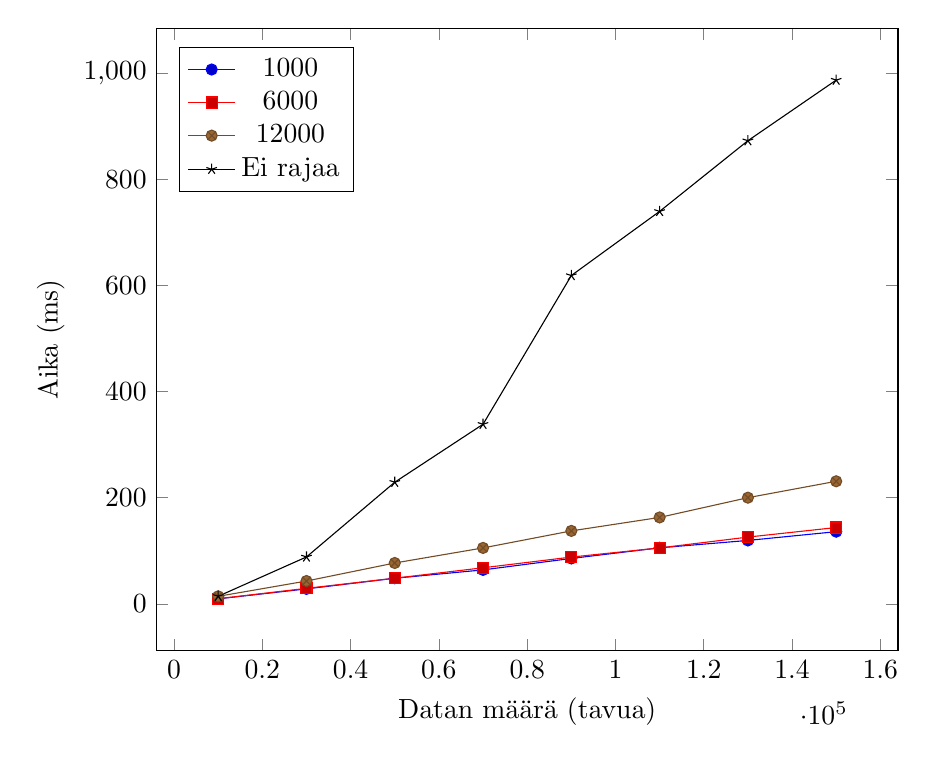
\begin{tikzpicture}
	\begin{axis}[
			xlabel=Datan määrä (tavua),
			ylabel=Aika (ms),
			legend pos=north west]
		
		\addplot coordinates {
			(10000,9.57)
			(30000,28.35)
			(50000,48.37)
			(70000,64.13)
			(90000,85.68)
			(110000,105.72)
			(130000,119.63)
			(150000,136.15)
		};
		\addlegendentry{1000}
		
		\addplot coordinates {
			(10000,9.87)
			(30000,29.34)
			(50000,48.48)
			(70000,68.10)
			(90000,88.29)
			(110000,105.50)
			(130000,125.92)
			(150000,143.95)
		};
		\addlegendentry{6000}

		\addplot coordinates {
			(10000,14.32)
			(30000,43.15)
			(50000,77.13)
			(70000,105.51)
			(90000,137.60)
			(110000,162.98)
			(130000,200.18)
			(150000,231.06)
		};
		\addlegendentry{12000}
		
		\addplot coordinates {
			(10000,14.43)
			(30000,88.49)
			(50000,229.31)
			(70000,338.52)
			(90000,618.74)
			(110000,739.59)
			(130000,872.75)
			(150000,986.94)
		};
		\addlegendentry{Ei rajaa}
		
	\end{axis}
\end{tikzpicture}
\caption{Pakkausnopeus satunnaisesti generoidulla datalla}
\end{figure}

Kuvasta nähdään hyvin, miten sanakirjan rajan poistaminen vaikuttaa pakkausnopeuteen --- testin perusteella se pysyy lineaarisena niin kauan kun sanakirjalla on jokin raja, mutta rajan poistaminen seurauksena pakkausnopeus hidastuu merkittävästi.

Syynä pakkauksen hidastumiseen nostaessa sanakirjan rajaa lienee hajautustaulun operaatioiden hidastuminen, kun siihen lisättyjen alkioiden määrä kasvaa.

Käyttämällä datana suomenkielistä tekstiä --- testiaineistona käytettiin Project Gutenbergistä löytyvää \emph{Seitsemän Veljestä}-kirjaa\footnote{\url{http://www.gutenberg.org/ebooks/11940}} --- saadaan kovin erinäköisiä tuloksia:

\begin{figure}[h]
\centering
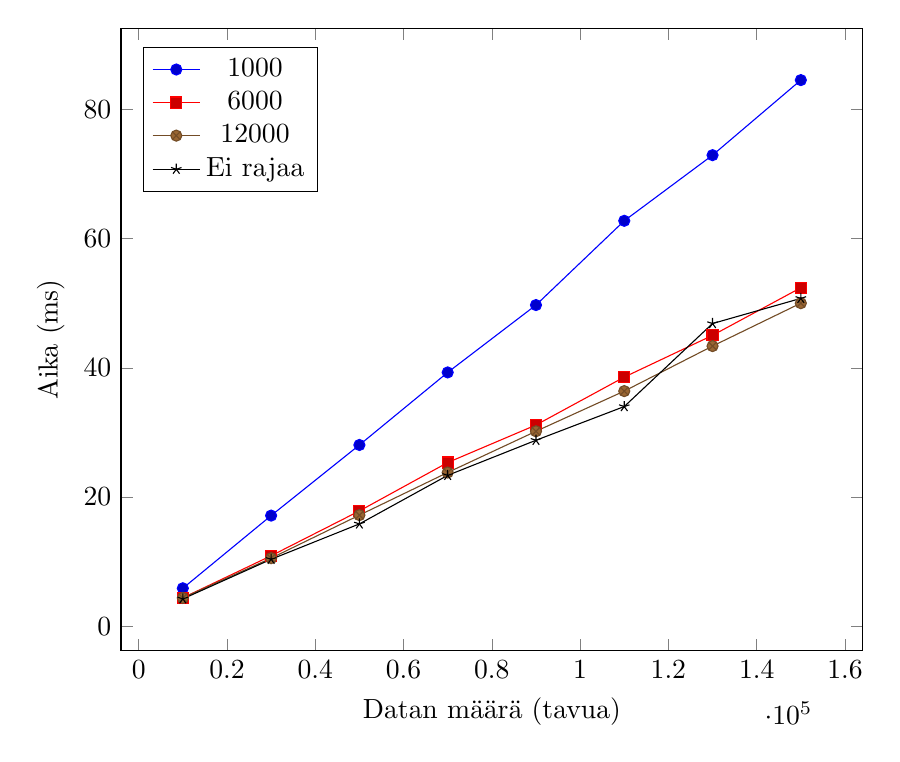
\begin{tikzpicture}
	\begin{axis}[
			xlabel=Datan määrä (tavua),
			ylabel=Aika (ms),
			legend pos=north west]
		
		\addplot coordinates {
			(10000,5.87)
			(30000,17.12)
			(50000,28.05)
			(70000,39.28)
			(90000,49.71)
			(110000,62.75)
			(130000,72.91)
			(150000,84.53)
		};
		\addlegendentry{1000}
		
		\addplot coordinates {
			(10000,4.39)
			(30000,10.90)
			(50000,17.84)
			(70000,25.33)
			(90000,31.14)
			(110000,38.56)
			(130000,45.02)
			(150000,52.39)
		};
		\addlegendentry{6000}

		\addplot coordinates {
			(10000,4.38)
			(30000,10.53)
			(50000,17.19)
			(70000,23.79)
			(90000,30.17)
			(110000,36.39)
			(130000,43.36)
			(150000,50.00)
		};
		\addlegendentry{12000}
		
		\addplot coordinates {
			(10000,4.23)
			(30000,10.36)
			(50000,15.83)
			(70000,23.35)
			(90000,28.78)
			(110000,34.00)
			(130000,46.85)
			(150000,50.74)
		};
		\addlegendentry{Ei rajaa}
		
	\end{axis}
\end{tikzpicture}
\caption{Pakkausnopeus suomenkielisellä tekstillä}
\end{figure}

150 000 tavua dataa ei välttämättä ole tarpeeksi että eri sanakirjan sanamäärän rajojen vaikutukset pakkausnopeuteen tulisivat esille, mutta liian pienellä rajalla pakkausnopeus kärsii huomattavasti --- satunnaisella datalla näin ei käynyt. Kenties hajautustaulun alkioiden määrä ei ylitä jotain rajaa, joka aiheuttaisi täyttöasteen pienenemisen ja hajautustaulun operaatioista tulisi nopeampia. Tai vaihtoehtoisesti hidasta uudelleenhajautusta joudutaan tekemään 1000 sanan rajalla jatkuvasti.

Purkunopeudessa yhtä merkittäviä eroja ei ole havaittavissa, vaikkakin sanakirjan rajan ja datan sisällön vaikutukset purkunopeuteen ovatkin samansuuntaisia kuin pakkausnopeuteen. Purkaminen on kuitenkin selkeästi pakkaamista nopeampaa, etenkin satunnaisella datalla.

\subsection{Pakkausteho}

\begin{figure}[h]
\centering
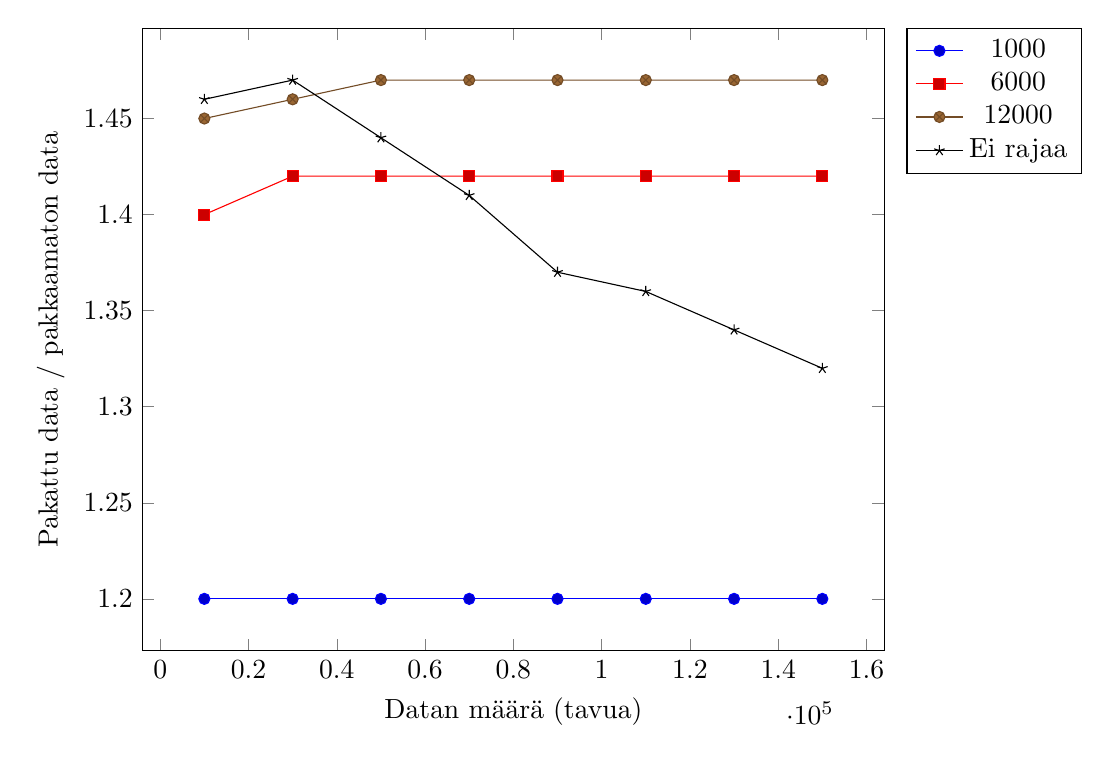
\begin{tikzpicture}
	\begin{axis}[	        
			xlabel=Datan määrä (tavua),
			ylabel=Pakattu data / pakkaamaton data,
			legend pos=outer north east]
		
		\addplot coordinates {
			(10000,1.2)
			(30000,1.2)
			(50000,1.2)
			(70000,1.2)
			(90000,1.2)
			(110000,1.2)
			(130000,1.2)
			(150000,1.2)
		};
		\addlegendentry{1000}
		
		\addplot coordinates {
			(10000,1.40)
			(30000,1.42)
			(50000,1.42)
			(70000,1.42)
			(90000,1.42)
			(110000,1.42)
			(130000,1.42)
			(150000,1.42)
		};
		\addlegendentry{6000}

		\addplot coordinates {
			(10000,1.45)
			(30000,1.46)
			(50000,1.47)
			(70000,1.47)
			(90000,1.47)
			(110000,1.47)
			(130000,1.47)
			(150000,1.47)
		};
		\addlegendentry{12000}
		
		\addplot coordinates {
			(10000,1.46)
			(30000,1.47)
			(50000,1.44)
			(70000,1.41)
			(90000,1.37)
			(110000,1.36)
			(130000,1.34)
			(150000,1.32)
		};
		\addlegendentry{Ei rajaa}
		
	\end{axis}
\end{tikzpicture}
\caption{Pakkaussuhde satunnaisella datalla}
\end{figure}

Ensimmäinen huomioitava asia satunnaista dataa pakattaessa on se, että kaikissa testatuissa tapauksissa pakkaussuhde on enemmän kuin 1 --- käytännössä tämä tarkoittaa sitä, että pakattu tiedosto on \emph{suurempi} kuin pakkaamaton tiedosto. Implementaatio ei siis sellaisenaan sovellu minkä tahansa datan pakkaamiseen, jos halutaan varmistaa että pakkaus ei kasvata tiedostokokoa.

Sanakirjan rajan muuttamisella on kuitenkin mielenkiintoisia seurauksia pakkaustehoon. Toisin kuin voisi kuvitella, sanakirjan rajan kasvattaminen --- joka siis mahdollistaa useampien aiemmin esiintyneiden datanpätkien esittämisen yhdellä koodilla --- ei parannakaan pakkaussuhdetta.

Ilmiö on selitettävissä sillä, että satunnaisessa datassa sanakirjasta löytyviä datanpätkiä ei käytännössä pystytä hyödyntämään lainkaan, sillä datassa ei esiinny toistuvia rakenteita. Samalla kuitenkin sanakirjaan luodaan hyvin paljon uusia data-koodi-pareja, joka aiheuttaa sen, että yhden koodin esittämiseen tarvittava bittimäärä kasvaa jatkuvasti. Jos raja on 1000, sanakirjassa ei koskaan ole sitä enempää data-koodi-pareja ja myös koodin esittämiseen tarvittava bittimäärä pysyy alhaisena. Rajalla 6000 yhden koodin esittämiseen tarvittava bittimäärä kasvaa korkeammaksi, kuitenkaan mitenkään hyötymättä sanakirjan suuremmasta koosta.

Vasta jos raja poistetaan kokonaan sanakirjassa on niin paljon data-koodi-pareja, että niitä voidaan käyttää pakkaamisen apuna. Näin myös pakkaussuhde paranee sitä mukaa mitä enemmän dataa pakataan. Kuten aiemmin todettiin, rajan poistaminen kuitenkin aiheuttaa pakkaamiseen kuluvan ajan räjähdysmäisen kasvun.

\begin{figure}[h]
\centering
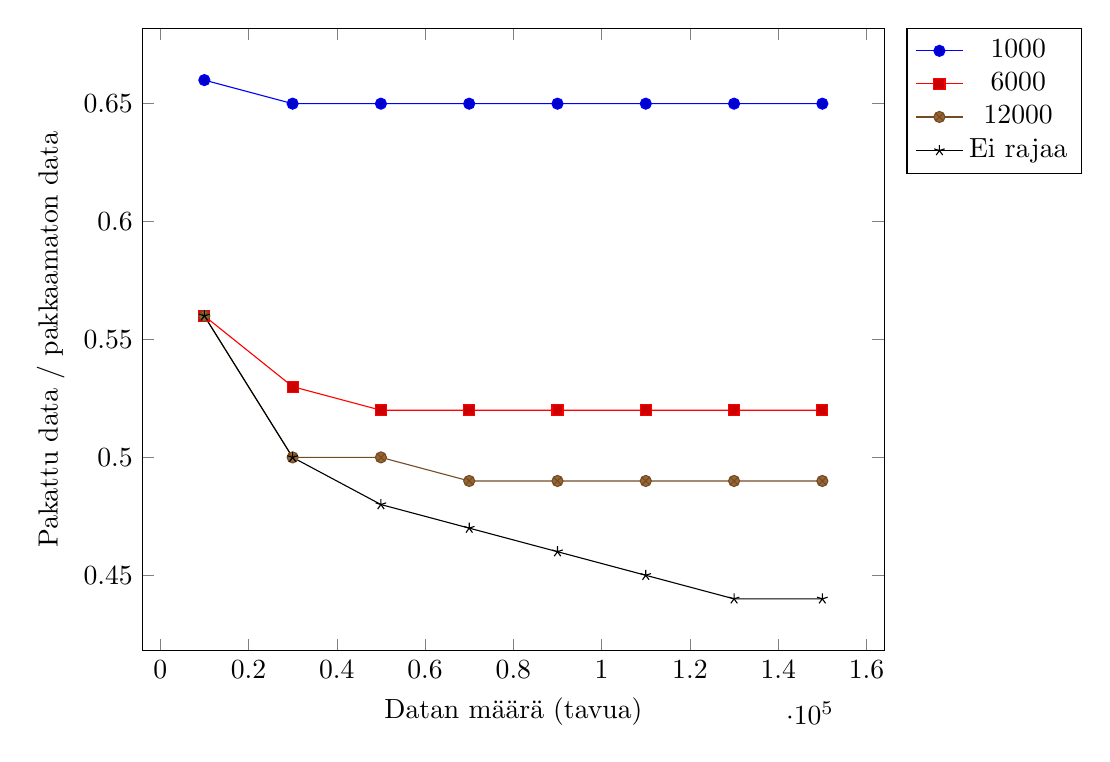
\begin{tikzpicture}
	\begin{axis}[	        
			xlabel=Datan määrä (tavua),
			ylabel=Pakattu data / pakkaamaton data,
			legend pos=outer north east]
		
		\addplot coordinates {
			(10000,0.66)
			(30000,0.65)
			(50000,0.65)
			(70000,0.65)
			(90000,0.65)
			(110000,0.65)
			(130000,0.65)
			(150000,0.65)
		};
		\addlegendentry{1000}
		
		\addplot coordinates {
			(10000,0.56)
			(30000,0.53)
			(50000,0.52)
			(70000,0.52)
			(90000,0.52)
			(110000,0.52)
			(130000,0.52)
			(150000,0.52)
		};
		\addlegendentry{6000}

		\addplot coordinates {
			(10000,0.56)
			(30000,0.50)
			(50000,0.50)
			(70000,0.49)
			(90000,0.49)
			(110000,0.49)
			(130000,0.49)
			(150000,0.49)
		};
		\addlegendentry{12000}
		
		\addplot coordinates {
			(10000,0.56)
			(30000,0.50)
			(50000,0.48)
			(70000,0.47)
			(90000,0.46)
			(110000,0.45)
			(130000,0.44)
			(150000,0.44)
		};
		\addlegendentry{Ei rajaa}
		
	\end{axis}
\end{tikzpicture}
\caption{Pakkaussuhde suomenkielisellä tekstillä}
\end{figure}

Hyvin pakkautuvalla datalla tulokset ovat sellaisia kuin voisi odottaa - sanakirjan rajan kasvattaminen ja lopulta poistaminen parantaa aina pakkaussuhdetta. Kuten satunnaisellakin datalla, käyttäessä sanakirjan rajaa pakkaussuhde ei parane pakattaessa enemmän dataa --- tämä johtuu sanakirjan jatkuvasta alustamisesta joka vuorostaan aiheuttaa sen, että aiemmin kerättyjä data-koodi-pareja ei voida hyödyntää sanakirjan resetoinnin jälkeen. Sanakirjan rajan poistaminen poistaa myös tämän ilmiön.

Parhaimmillaan testeissä päästiin pakkaussuhteeseen 0.44, joka siis tarkoittaa, että pakattu tiedosto on 44\% alkuperäisen tiedoston koosta.

\end{document}